\documentclass{article}

% Indicamos que el lenguaje es el español 
\usepackage[spanish]{babel} % Soporte multilenguaje para LaTeX.
\usepackage[a4paper, top=2.5cm, bottom=2.5cm, left=2.5cm, right=2.5cm]{geometry} % Interfaz flexible para definir las dimensiones del documento
\usepackage[utf8]{inputenc} % Aceptar diferentes tipos de codificación de caracteres de entrada (en este caso usamos la codificación Unicode UTF-8)
\usepackage{graphicx} % Soporte aumentado para gráficos 
\usepackage{color} % Para usar colores
\usepackage{hyperref} % Para manejar referencias cruzadas. P.ej. añadir hiperenlaces al índice





\begin{document}
	
	\begin{titlepage}
		
		\begin{center}
			\vspace*{0.1in}

			
			FACULTAD DE INFORMÁTICA\\
			\vspace*{0.55in}
				
			\begin{figure}[htb]
							\begin{center}
								
\includegraphics[width=8cm]{./logo.png}
							\end{center}
			\end{figure}
			\vspace*{0.8in}
			\large Diseño de Redes\\
			\vspace*{0.4in}
			\begin{Large}
				\textbf{MEMORIA DE PRÁCTICAS} \\
			\end{Large}
			\vspace*{2.5in}
			\begin{large}
				Curso 2015 - 2016\\
			\end{large}
			\rule{80mm}{0.1mm}\\
			
			\begin{large}
				Alumnos \\
				Brais López Chao\\
				Miguel Pérez Rego\\
			\end{large}
		\end{center}
		
	\end{titlepage}

	
	\pagenumbering{arabic}
	\tableofcontents
	\newpage
	
	\section{Práctica 1}
	
	\subsection{Tutorial de OMNeT++}
	
		\subsubsection{Ejemplo 6}
		
		Se muestra el manejo de la temporización en los mensajes. Básicamente lo que hace el módulo es reenviarse el mensaje a sí mismo con un tiempo de retardo. Para esto, primero se declaran en \textit{txc6.cc} las variables \textit{event}, y \textit{tictocMsg}. Lo que se va a usar ahora es la función \textit{ScheduleAt}. Cuando esta es llamada por un módulo se reenvía a sí misma el evento que le pasemos con un delay indicado. Así, gracias a un if, si en el mensaje que recibe un módulo viene un evento, quiere decir que es recibido del mismo módulo, por lo que lo enviamos a fuera. Si es recibido de un módulo distinto, se schedulea para esperar x tiempo.
		
		\subsubsection{Ejemplo 7}
		
		En el ejemplo 7 empezamos a analizar valores aleatorios. Para eso, declaramos dos variables, que las podemos poner en el omnetpp.ini, o en el tictoc7.ned. Esta variable se denominará delaytime.
		
		Ahora, cuando tengamos un mensaje recibido de fuera, en lugar de retrasarlo 5 segundos, lo retrasaremos un delaytime aleatorio, que también varía dependiendo de si es tic o toc el módulo que lo recibe.
		
		Por último, también se añade una función uniform, que depende del valor que sea, descarta el mensaje cuando sea menor de 0.1.
		
		\subsubsection{Ejemplo 8}
		
		En este caso lo que hacemos es cambiar el comportamiento de tic y toc. 

		En el caso de tic, cuando se envía un mensaje, se establece un tiempo de timeout mediante un schedule message, de manera que estamos enviando dos mensajes realmente, uno para toc y otro para nosotros mismos. En caso de que llegue antes el de timeout, significará que el timeout ha pasado, y reenviaremos el mismo mensaje (nuevo). En caso de que llegue antes el paquete, de toc, significará que no ha pasado el timeout, en cuyo caso hay que cancelar el mensaje de timeout, y enviar una respuesta  toc.
		
		Ahora, el comortamiento toc es similar al anterior, lo que hace es establecer una probabilidad de fallo, y en caso de que no falle reenvia un mensaje y todo correcto.
		
		\subsubsection{Ejemplo 9}
		
		En este ejemplo, se va a hacer lo mismo que en el ejemplo 8, pero reenviando el mismo mensaje en caso de pérdida. Para ello se crean varias variables globales, una donde se almacenará el mensaje que se está enviando, que es *message, y otra que es el número de secuencia para incrementar el contador de cada vez que se reenvie un mensaje y que sean todos distintos.
		
		En tic, cuando se envía un mensaje, se guarda la copia de dicho mensaje con message=generatenewmessage(). Este mensaje será el que enviemos, junto con un scheduled a nosotros mismos. Si llega antes el scheduled, tendremos que reenviar este message en variable global, para ello usamos sencopyoff, una función que reenvía el mismo mensaje de la variable global, ya uqe la función generatenewmessage crea uno nuevo de cada vez. En caso de que llegue antes el mensaje que el timeout, se repite el proceso con un generatenewmessage.
		
		El comportamiento de toc es idéntico, pero sin olvidarse de limpiar cada msg de cada vez, para uqe no se nos acumulen, ya que son todos distintos.
		
		\subsubsection{Ejemplo 10}
		
		En este ejemplo se cambia completamente el comportamiento de la red. Ahora nuestra red tendrá varios nodos, especificados en el tictoc10.ned como una matriz. Lo bueno es que cada nodo tiene el mismo comportamiento, que es el siguiente: si la función getindex, que nos dice que número de nodo es el que la ejecuta, da igual al valor que predeterminamos en handle message, se acaba la simulación. Si no es igual, se envía por una de las puertas de salida del nodo, de modo aleatorio, por lo que el mensaje dará vueltas continuamente hasta encontrar el nodo al que se refiere.
		
		Con este comportamiento se puede implementar funcionalidades mas complejas que se ven en el ejemplo 11.
		
		\subsubsection{Ejemplo 11}
		
		En el ejemplo 11 vamos a cambiar solo el .ned. En la definición del canal, o sea, lo que conecta un nodo con otros, se va a utilizar un canal predefinido al principio con un valor único para el delay, que heredará de ned.delaychannel, que es un tipo de canal ya definidio en el paquete ned. Así podremos cambiar el delaychanel entero sin tener que seleccionar cada canal individualmente.
		
		\subsubsection{Ejemplo 12}
		
		En este ejemplo se muestra el funcionamiento de inoutgate, de manera que no tenemos que tener dos canales independientes, uno de ida y otor de vuelta, sino que funcionaremos solo con uno de ida y vuelta.
		
		También, en el .cc se cambiará la denominación de out cuando se envía , por gate simplemente, con el sufijo \$o o \$i para indicar si estamos usando una pierta de entrada o una de salida.
		
		\subsubsection{Ejemplo 13}
		
		En este ejemplo cambiará totalmente el funcionamiento del mensaje. Lo primero de todo es crear una clase .msg, con los campos que requerirá nuestor mensaje, esto es, un número de hops, o contador, un destino, y un origen, para así guardar todos los datos dentro del  mensaje.
		
		En el .cc, cambiará el comportamiento de cada nodo, de manera que se crea un mensaje con un destino y un origen, y va por las puertas aleatoriamente hasta llegar al destino, que se convertirá en nodo origen creando un nuevo mensaje con un nuevo destino aleatorio, de manera infinita. Por ahora, la puerta por la que van saliendo los mensajes seguirá siendo aleatoria.
		
		\subsubsection{Ejemplo 14}
		
		Lo primero que se va a implementar en este ejemplo son dos varíables globales numsend y numrecibed, que se usarán para crear un contador en cada nodo del número de mensajes que le han llegado y del número que han recibido.
		Cuando se inicializa un módulo, en el inicialize, se ponen dichas variables a 0 y se usa la función watch en ellas.
		
		Ahora, siempre que un mensaje llegue a su destino, hay que aumentar el contador con  numsend++ y numrecibed++, de manera que se nos mostrará un cuadradito con los contadores en el simulador.
		
		\subsubsection{Ejemplo 15}
		
		En este ejemplo se implementarán las estadísticas, añadiendo al omnetpp.ini esta variable record-eventlog = true, y luego añadiendo dos variables hopcountstats y hopcountvector. Estas variable se actualizan con record y collect cuando llega un mensaje a cada sitio.
		
		Todas estas variables se llamarán en una nueva función que creamos, la finalize, que se invoca cuando termina la ejecución. Así, al finalice se nos mostrarán todas las stats recogidas.
	
		\subsubsection{Ejemplo 16}
		
		En este ejemplo, se reemplazarán las variables de estadística que creamos antes por un tipo de variable propia de omnet que son las señales. Estas guardarán las estadísticas de nuestra simulación.	Primero, en el .ned se declararán @signal y @stadistic. Luego en omnetpp.ini necesitaremos añadir ciertos valores para guardar las estadísticas.
		
		El gran cambio está en el archivo .cc, donde ya no necesitaremos las variables creadas anteriormente, si no que usaremos una variable de tipo simsignal, que guardará todo. Así , en el inicialice se registrará esta variable, y cuando llega a destino, con la función emit, le indicaremos a la señal que ha subido el contador. Tan sencillo como eso. 
		
		Por último, para analizar estos resultados almacenados por las señales tendremos que utilizar el ResultAnalizer tool.
		
		\newpage
		
		\subsection{Realización de la práctica}
		\subsubsection{Código}
		
		
		Lo primero que se ha hecho es crear una red Tictoc17 similar a la red Tictoc16. Para ello, se ha añadido al fichero \textit{omnetpp.ini} las siguientes lineas:\\
		
		\begin{figure}[htbp]
		\centering
		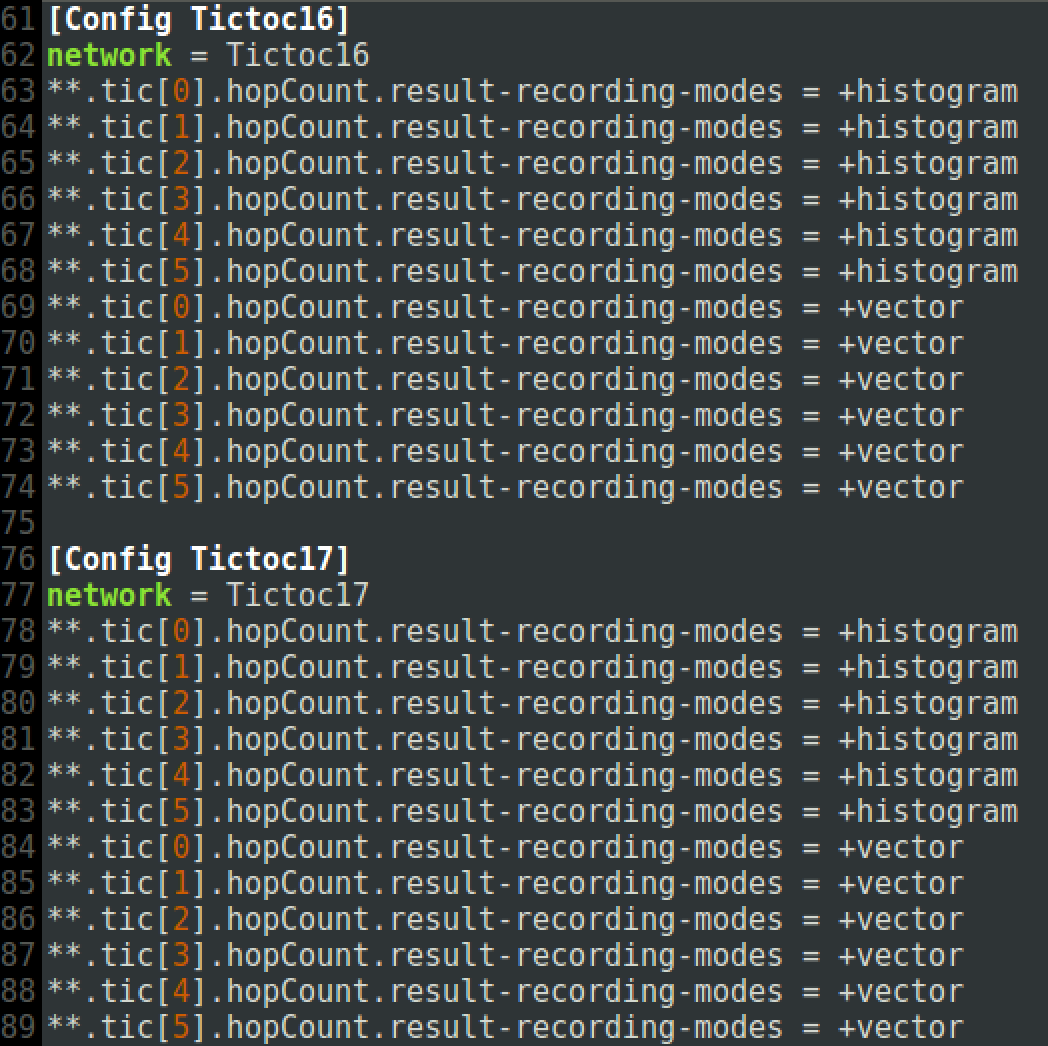
\includegraphics[width=0.9\textwidth]{figura1.png}
		\caption{Código tictoc17}
		\end {figure}
			
	
		Tras ello, se crean \textit{tictoc17.ned} y \textit{txc17.cc} idénticos a \textit{tictoc.ned} y \textit{txc16.cc} respectivamente. Será en \textit{txc17.cc} donde se harán las modificaciones pertinentes para las dos mejoras implementadas.
		
		En la primera mejora, se ha programado una implementación en la que un paquete no pueda salir por la misma puerta por la que llega a un nodo (exceptuando el caso en caso en el que el nodo solo tenga una puerta).Esto evita uno de los grandes problemas del funcionamiento de la red, la entrada en bucles erróneos antes de llegar a su destino.
		
		Para ello se han realizado las siguientes modificaciones en el fichero \textit{txc17.cc}:
		
		\newpage
		
		\begin{figure}[htbp]
		\centering
		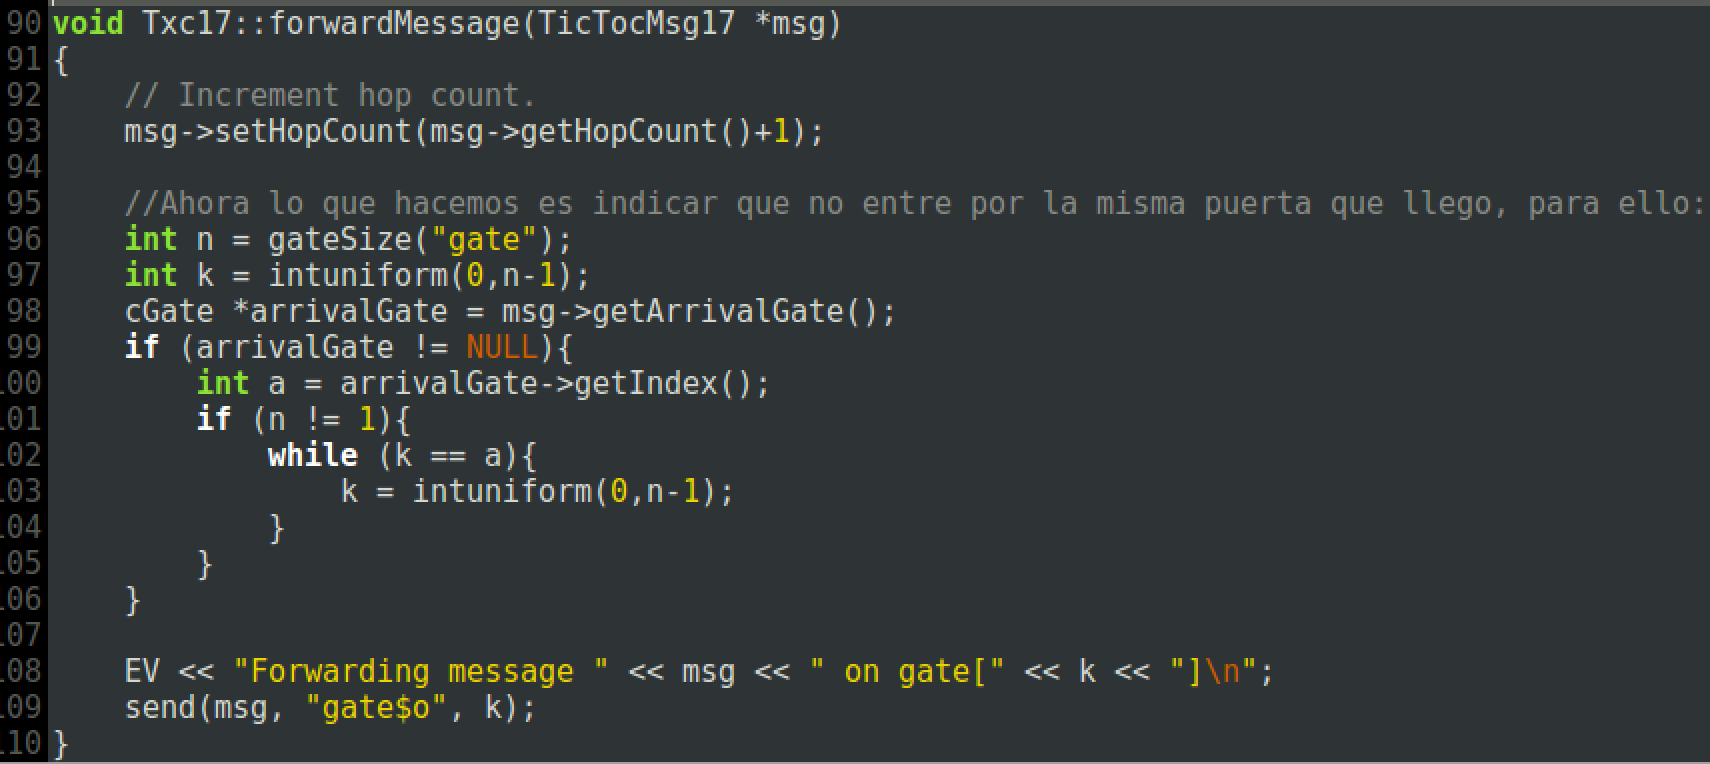
\includegraphics[width=0.9\textwidth]{figura2.png}
		\caption{Código tictoc17 v1}
		\end {figure}
			
		
		Como se aprecia en la figura, se ha utilizado la función \textit{getArrivalGate()} para obtener una instancia de la puerta por la que llega el mensaje. Una vez obtenida dicha puerta, con \textit{getIndex()} se guarda el número de  puerta qué es. Sabiendo el número de puerta, el mensaje no saldrá por ella siempre y cuando haya otra puerta por la que ir.\\
		
		Ahora bien, el comportamiento podría ser mejor, por lo que se ha decidido implementar una segunda mejora en la que se aprecien mejores resultados, ya que aún siguen existiendo bucles innecesarios.
		
		Para esta nueva mejora, se declararán dos nuevas variables en cada nodo: \textit{lastMessage} (guarda el identificador del último paquete que un nodo ha recibido) y \textit{lastGates} (un array que guarda un valor por cada puerta de cada uno de los nodos existentes, indicando si ya ha salido el mensaje o no por ella). 
		
		El funcionamiento del array \textit{lastGastes} es el siguiente: el valor 1, significará que el mensaje ya ha salido por esa puerta, y 0 en caso contrario. Así, se guardará información de por donde ha ido el mensaje, de manera que el programa realiza mejores elecciones en lugar de depender totalmente de la aleatoreidad. Con esto se evitan muchas repeticiones innecesarias y se mejora bastante el comportamiento del algoritmo, haciéndolo mucho mas predecible.Hay que tener en cuenta, que puede llegar un punto en el que todos los valores del array en un nodo estén a 1, en este caso se renicializarán todo, permitiendo salir en mensaje por cualquiera de las puertas (de esta forma se evitaría la perdida de mensajes en ciertas ocasiones).
		
		Cuando un mensaje llegue a su destino se reinicializará a 0 todos los valores de las puertas de los nodos, empezando así una nueva ejeución del proceso completo.\\
		
		La función de forwardMessage, recoge las nuevas mejoras implementadas:
		
		\begin{figure}[htb]
		\centering
		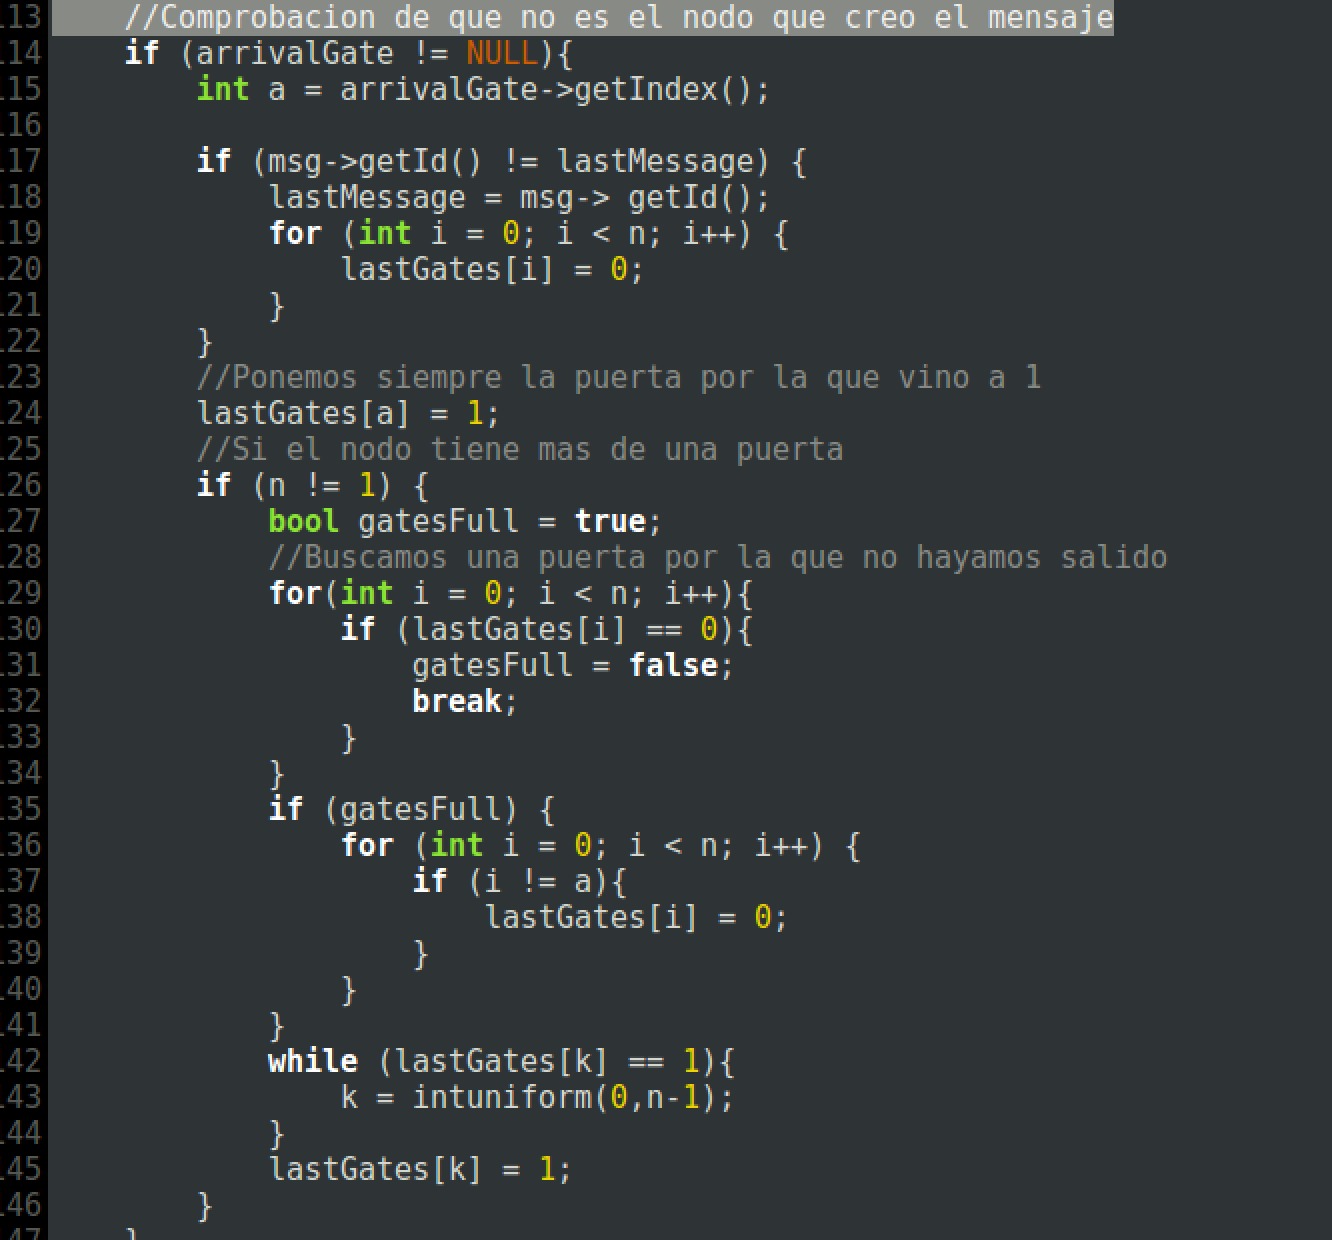
\includegraphics[width=0.9\textwidth]{figura3.png}
		\caption{Código tictoc17 v2}
		\end {figure}
		\newpage
		
		Estas son todas las mejoras que se han implementado. \\
		
		\subsubsection{Gráficas}
		
		Ahora se muestra la comparativa de las tres implementaciones, de manera que se puedan apreciar las mejoras implementadas. Se mostrarán cada gráfica respectivamente para las tres implementaciones, para ver en cada caso como los estos sencillos cambios actuan sobre la red tictoc.
		
		Para entender las gráficas es importante destacar que en nuestra simulación hay dos tipos de nodos a diferenciar: los nodos intermedios y los nodos externos.
		
		En nuestro caso los nodos intermedios serán tic1 y tic4, y los externos serán tic0, tic2, tic3 y tic5. Básicamente, los nodos intermedios tendrán un número medio de saltos antes de llegar a destino menor que los nodos externos, de manera que el comportamiento para cada caso es distinto y para llegar a un nodo intermedio se tendrá un número de saltos menor que a uno externo. Todo esto se apreciará en las siguientes gráficas.\\
	
		\newpage
		
		\textbf{Primera gráfica: dispersión de saltos en tic0 vs tic1}\\
	
		
		\begin{figure}[htb]
		\centering
		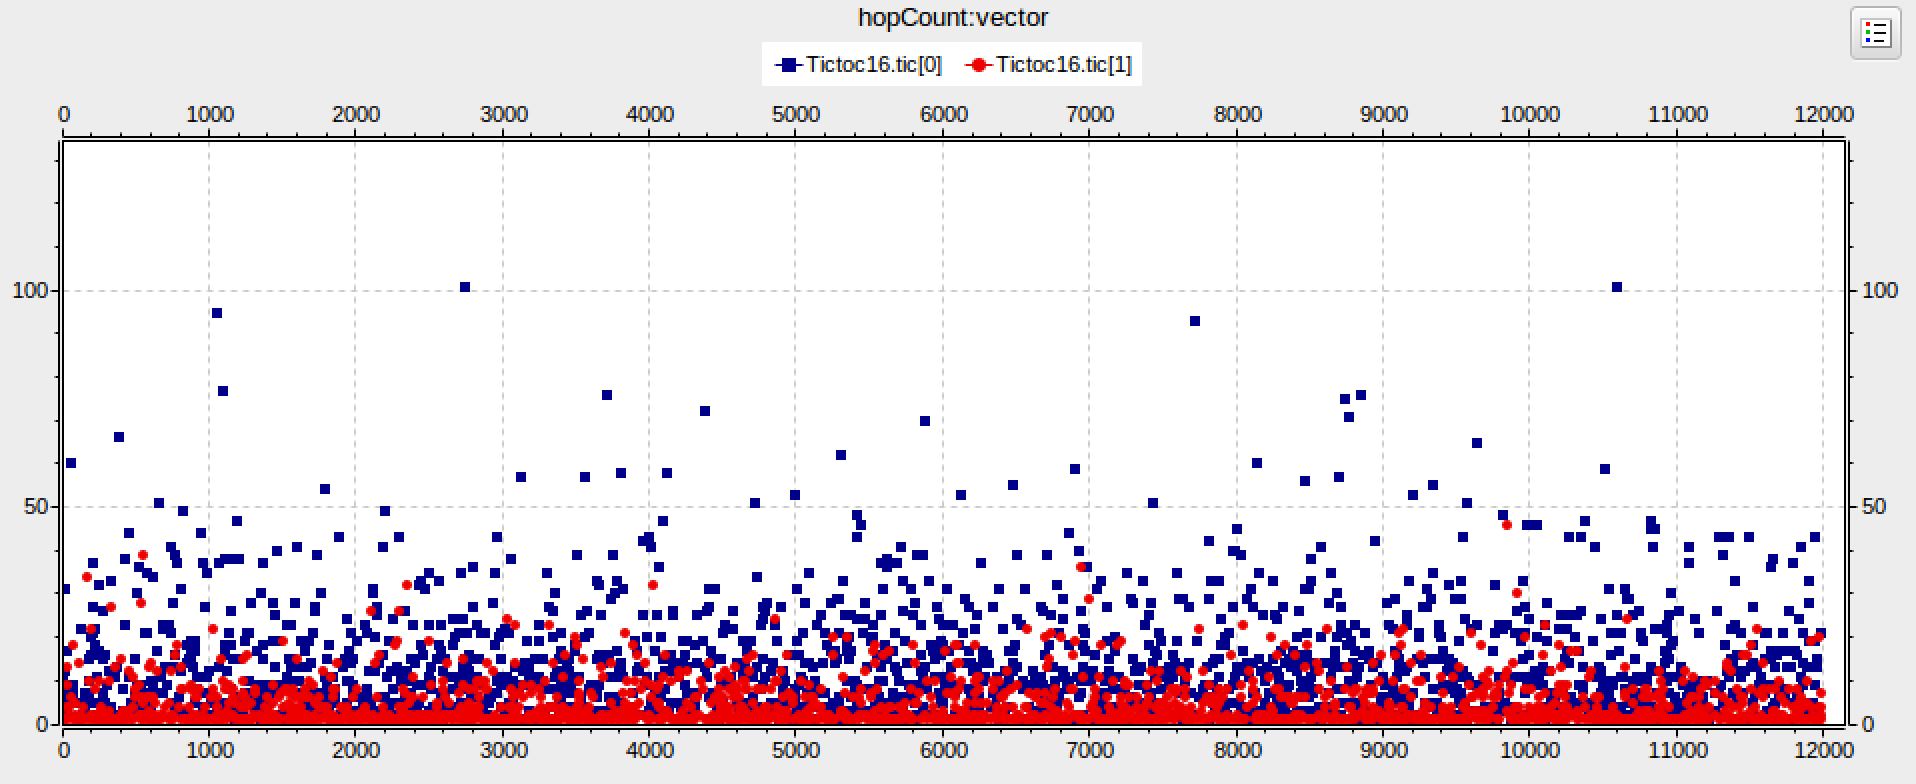
\includegraphics[width=0.9\textwidth]{tictoc16/figura1.png}
		\caption{Dispersión tictoc16}
		\end {figure}
		
		\begin{figure}[htb]
		\centering
		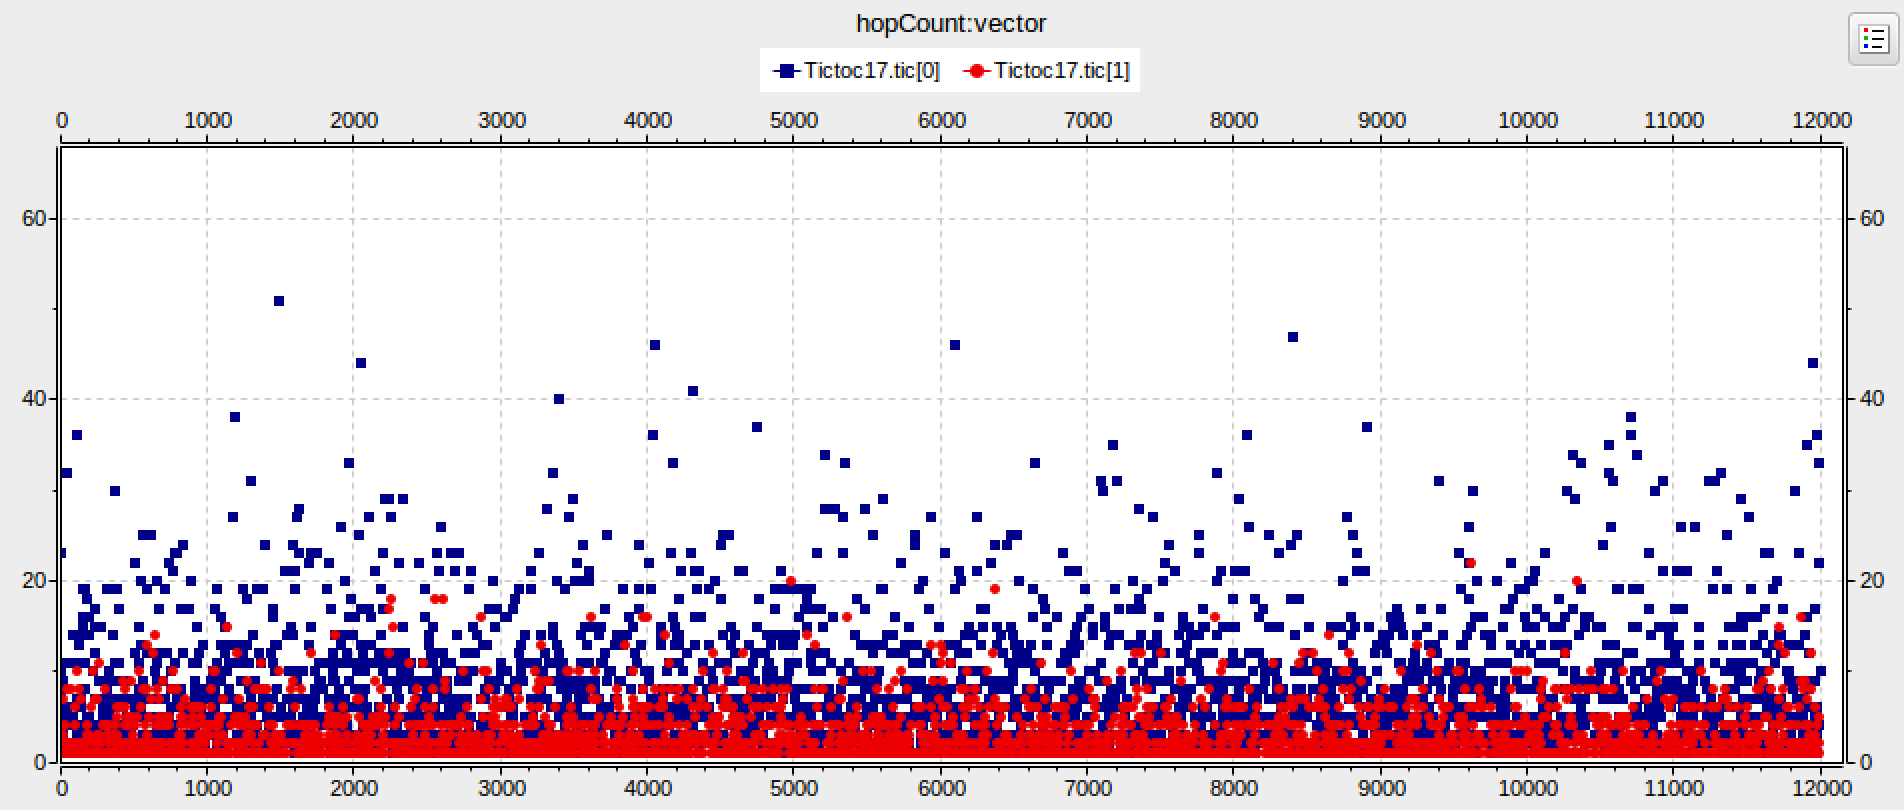
\includegraphics[width=0.9\textwidth]{tictoc17v1/figura1.png}
		\caption{Dispersión tictoc17 version 1}
		\end {figure}

		\begin{figure}[htb]
		\centering
		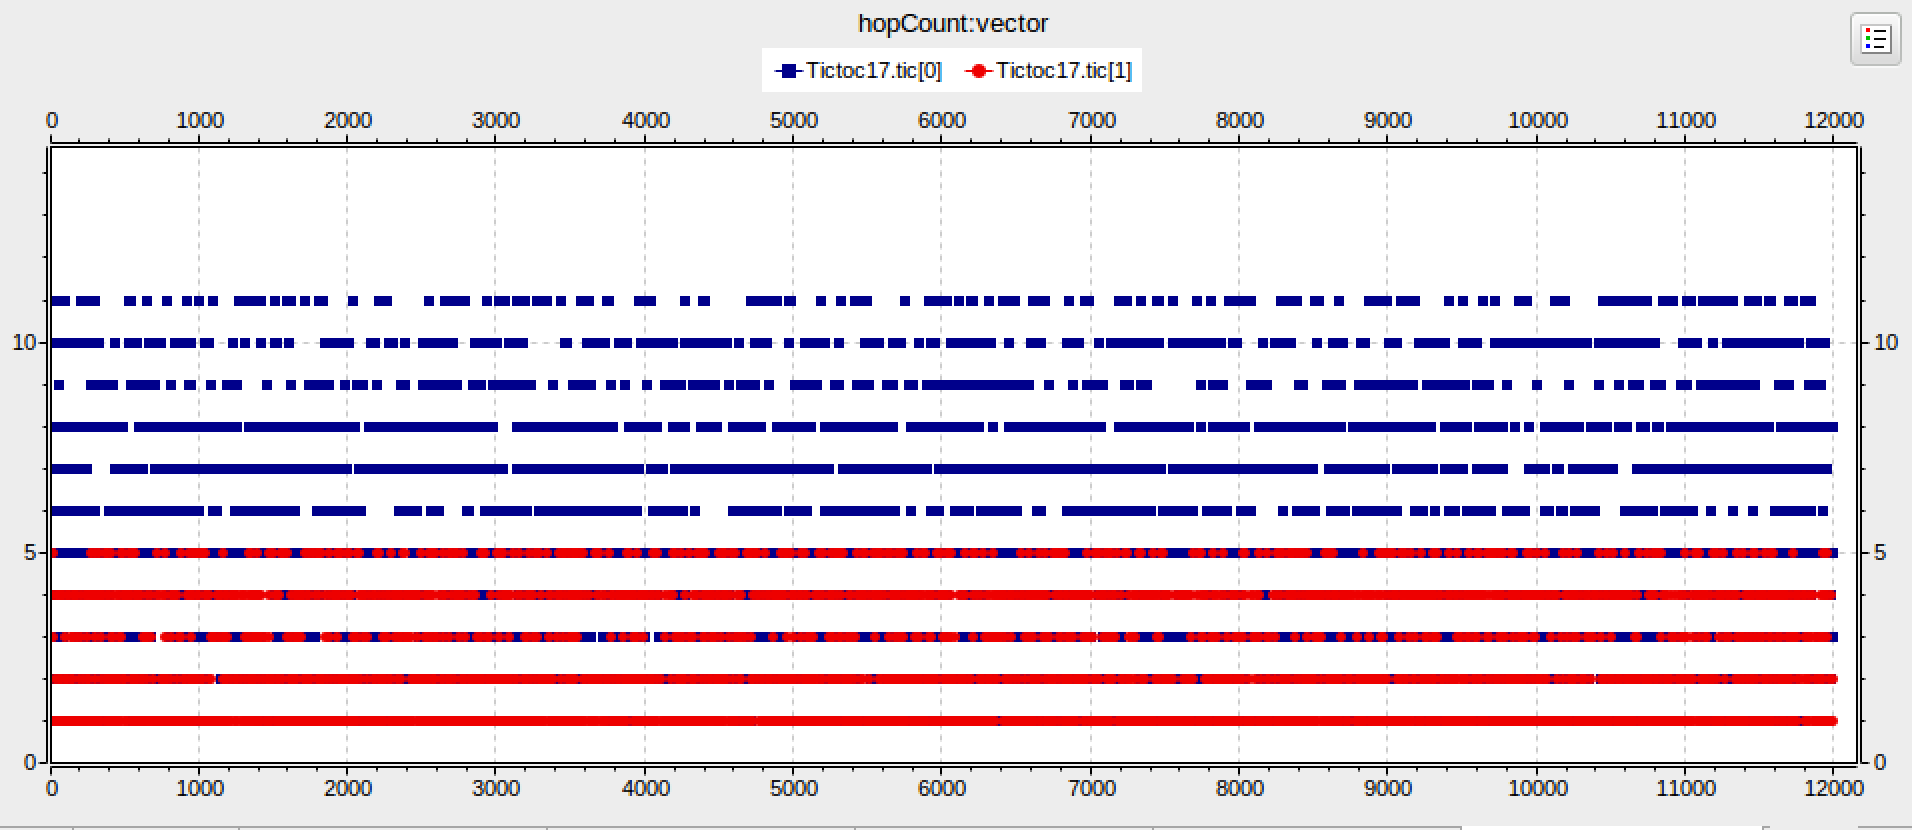
\includegraphics[width=0.9\textwidth]{tictoc17v2/figura1.png}
		\caption{Dispersión tictoc17 version 2}
		\end {figure}
		\newpage
		
		Como se puede apreciar en estas gráficas, la diferencia de saltos entre el nodo0, que es un nodo externo, y el nodo 1, que es un nodo intermedio es considerable.
		
		El principal problema que se aprecia es la aparición de puntos con muchos saltos repetidos antes de llegar al destino, que se producen por culpa de bucles en la ejecución. 
		
		Con la primera mejora bajamos bastante los puntos máximos a los qe se llegaba de 101 a 52. Sin embargo, con la versión dos de la mejora la dispersión es totalmente constante. De esta manera, un mensaje tardará en llegar a un nodo intermedio como mínimo 1 salto y como máximo máximo 5 saltos. Por su parte, a un nodo externo se llegará como mínimo a un salto y como máximo 11 saltos, lo que significa una mejora considerable en fiabilidad, de esta manera no se pierde tanto tiempo dando saltos innecesarios entre nodos.\\
		
		\textbf{Segunda gráfica: media de saltos por nodo}\\
		
		
		\begin{figure}[htb]
		\centering
		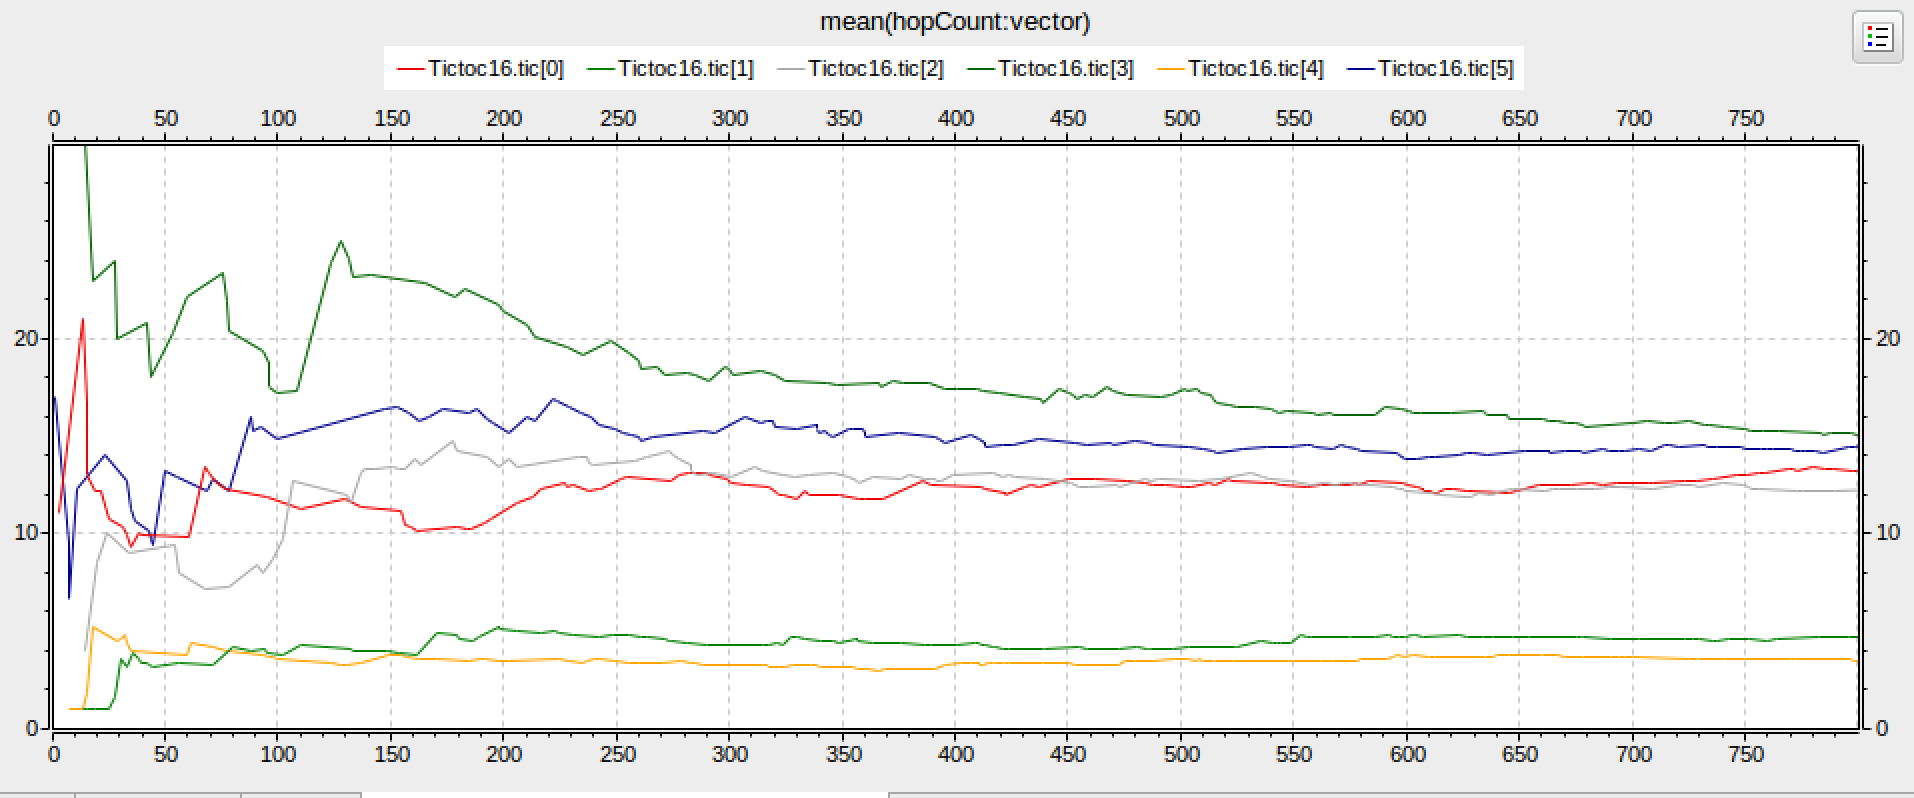
\includegraphics[width=0.9\textwidth]{tictoc16/figura2.png}
		\caption{Media tictoc16}
		\end {figure}
		\newpage
		
		\begin{figure}[htb]
		\centering
		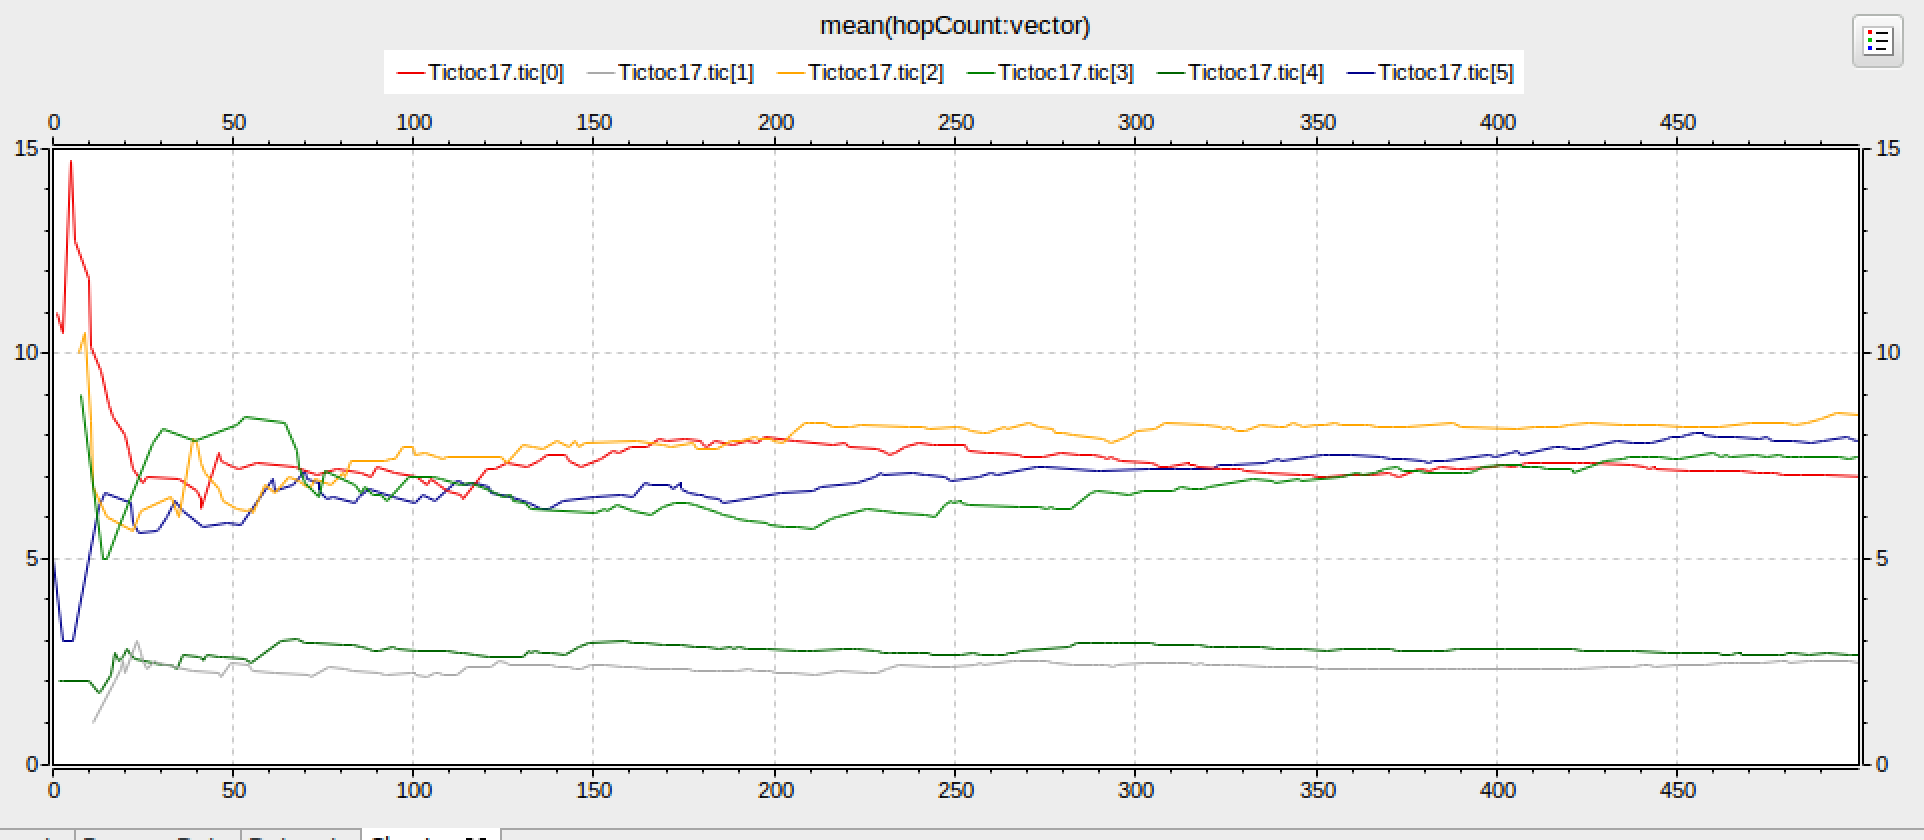
\includegraphics[width=0.9\textwidth]{tictoc17v1/figura2.png}
		\caption{Media tictoc17 version 1}
		\end {figure}

		\begin{figure}[htb]
		\centering
		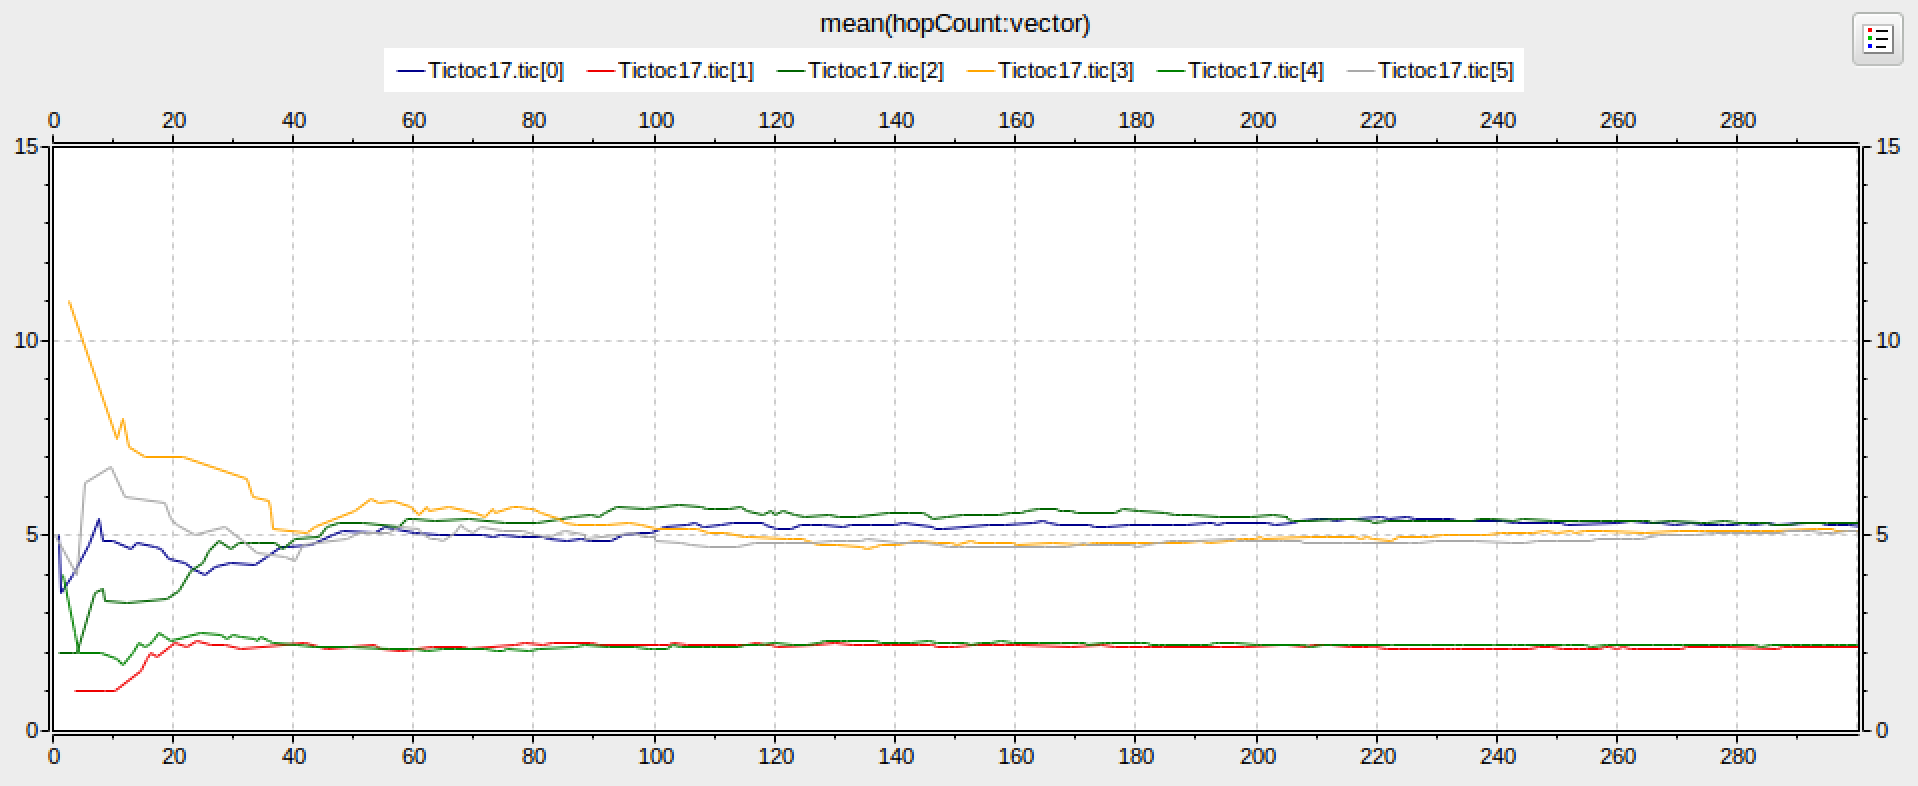
\includegraphics[width=0.9\textwidth]{tictoc17v2/figura2.png}
		\caption{Media tictoc17 version 2}
		\end {figure}

		Aquí se puede apreciar que en una ejecución larga, el número de saltos llega a una media similar para todos los nodos externos, y a otra para todos los nodos internos. La media de saltos para los nodos intermedios es menor que para los externos en cada implementación. Con la sprimera mejora se conisgue que lbaje el nímero de saltos bastante. Pese a esto, con la segunda mejora se supera aun ese margen, consiguiendo una media de 5 para los externos y 2 para los intermedios, lo cual denota un comportamiento muy estable de la red a largo plazo.\\
	
		\newpage
		
		\textbf{Tercera gráfica: histograma con el máximo y la media de saltos por nodo}\\
	
		\begin{figure}[htb]
			\centering
			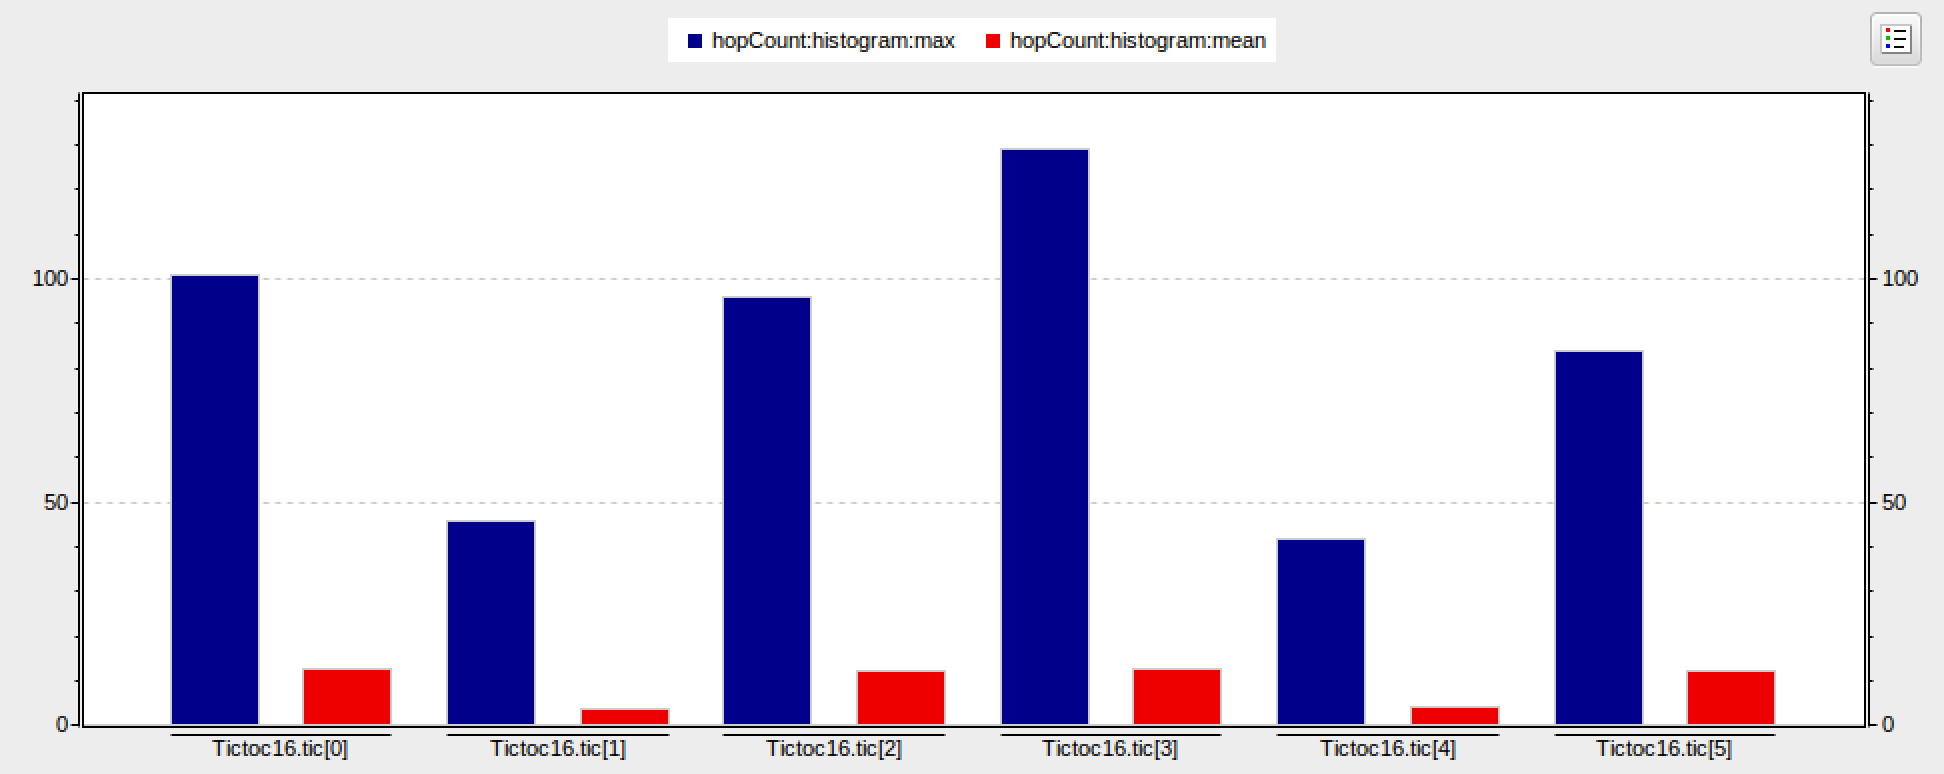
\includegraphics[width=0.9\textwidth]{tictoc16/figura3.png}
			\caption{Máximo y media por nodo tictoc16}
			\end {figure}
		
		\begin{figure}[htb]
			\centering
			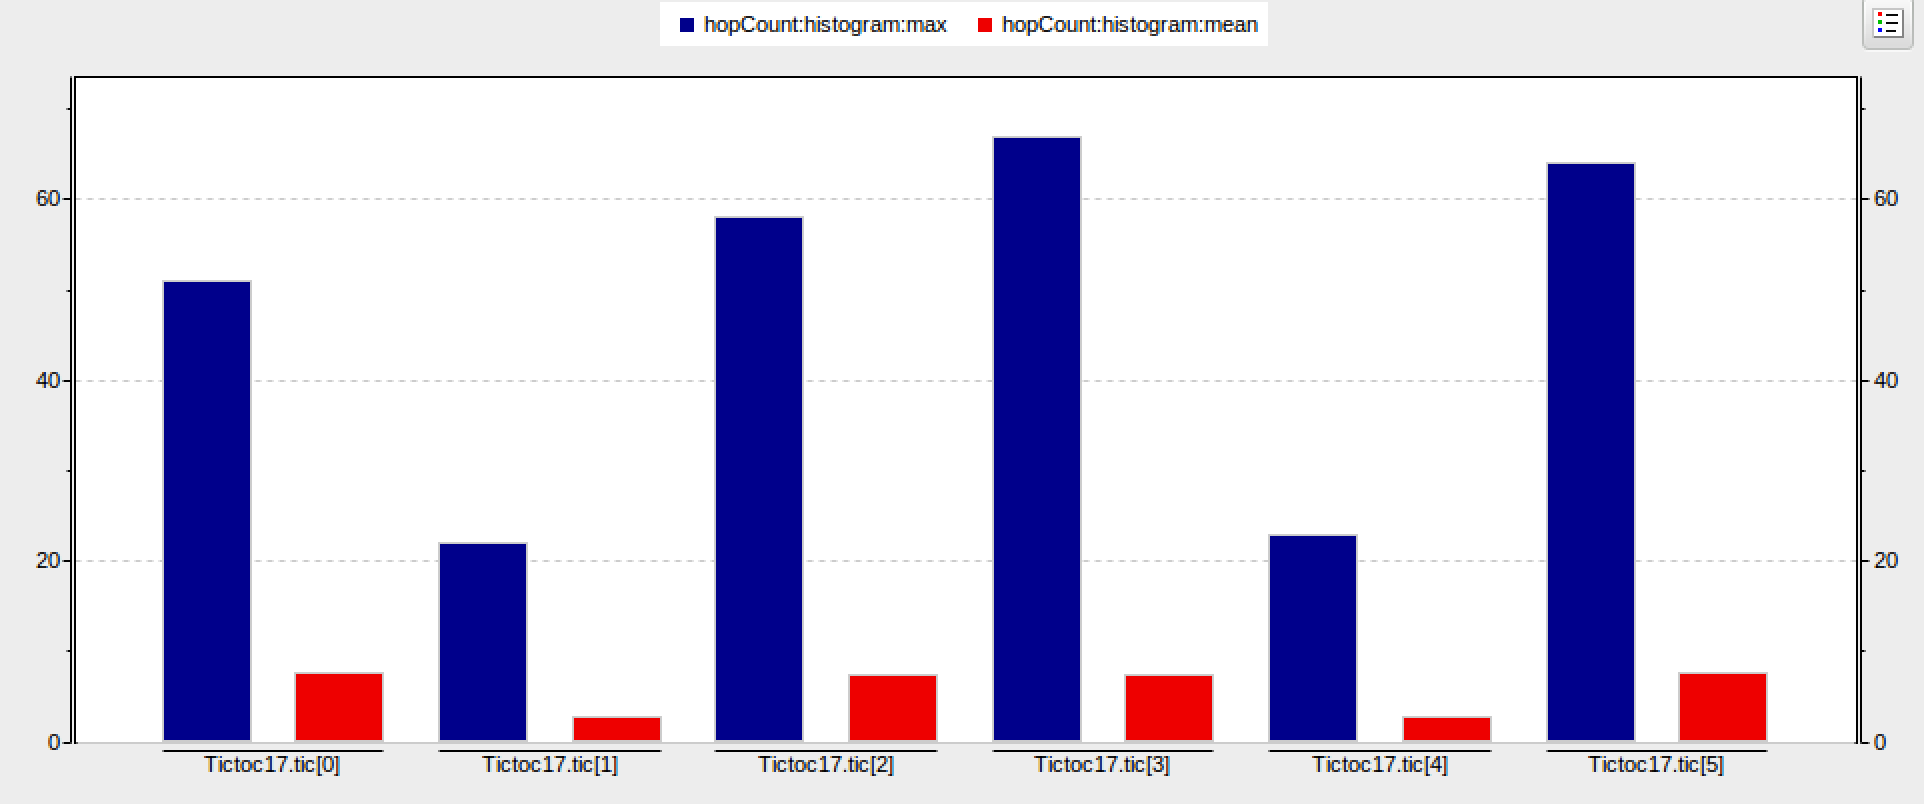
\includegraphics[width=0.9\textwidth]{tictoc17v1/figura3.png}
			\caption{Maximo y media por nodo tictoc17 version 1}
			\end {figure}

		\newpage
		\begin{figure}[htb]
			\centering
			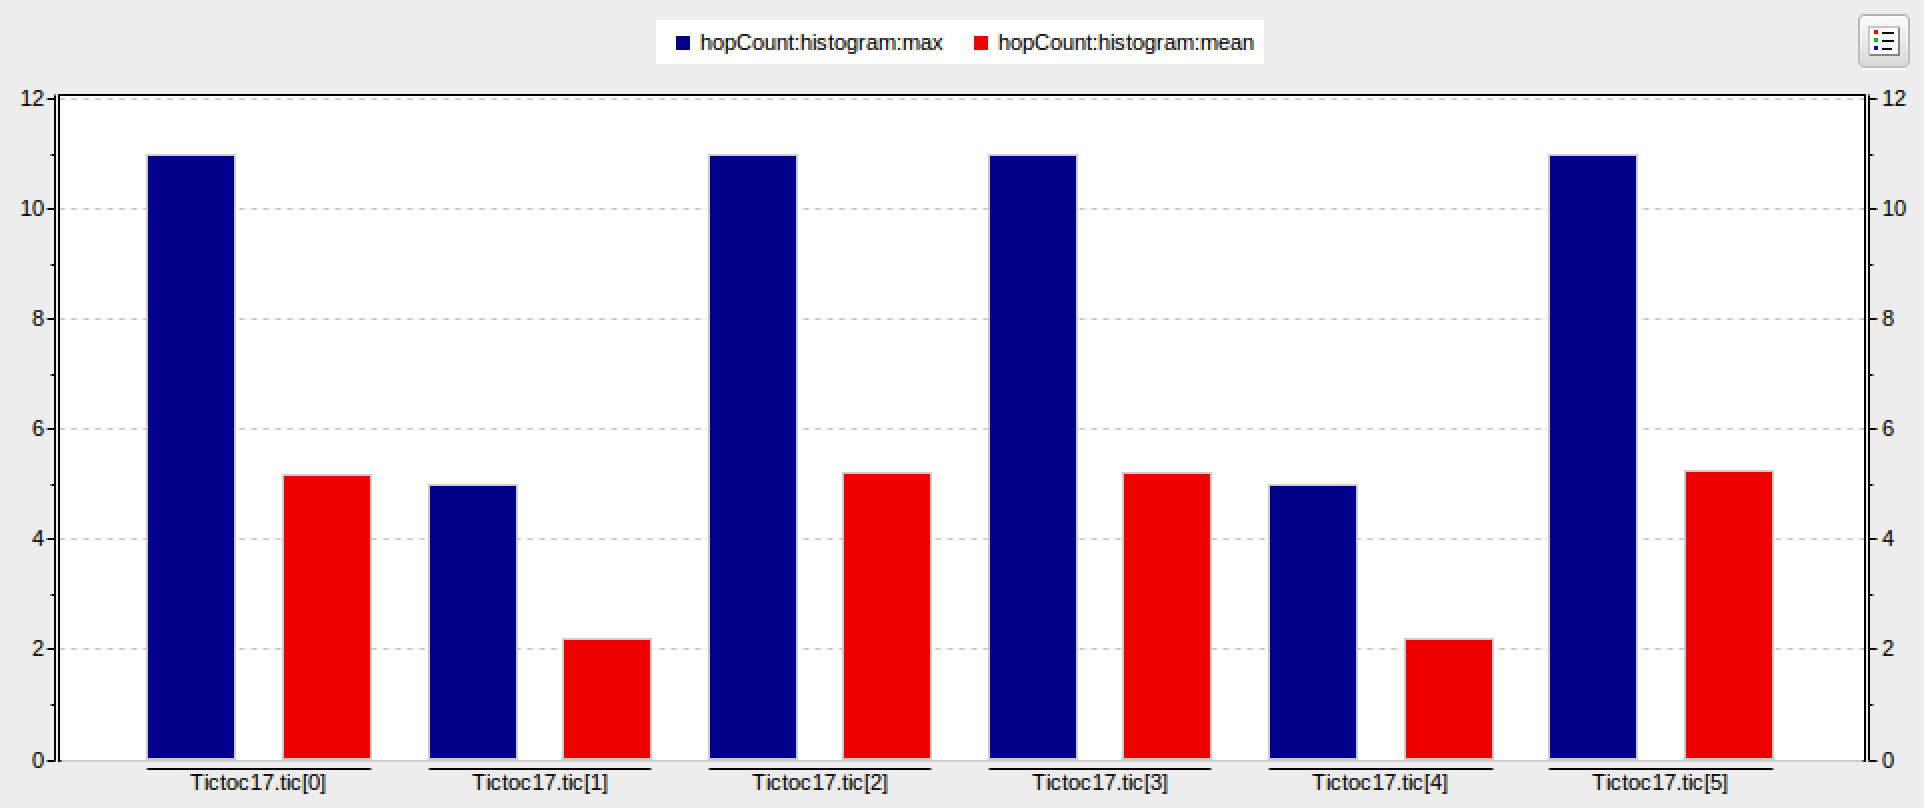
\includegraphics[width=0.9\textwidth]{tictoc17v2/figura3.png}
			\caption{Máximo y media por nodo tictoc17 version 2}
			\end {figure}
			
			
		Aquí se vuelve a apreciar la diferencia entre los nodos intermedios y los externos. El máximo con la segunda implementación de mejora baja hasta 11 en externos y 5 en intermedios, lo que permite que la media se coloque en 5 y 2 respectivamente. Con las implementaciones anteriores el máximo era mucho mas alto debido a los bucles lo que empeoraba el funcionamiento por falta de constancia.\\
		
		
		\textbf{Cuarta gráfica: histograma con las repeticiones del número de saltos en tic0, nodo externo}\\
		
		\begin{figure}[htb]
			\centering
			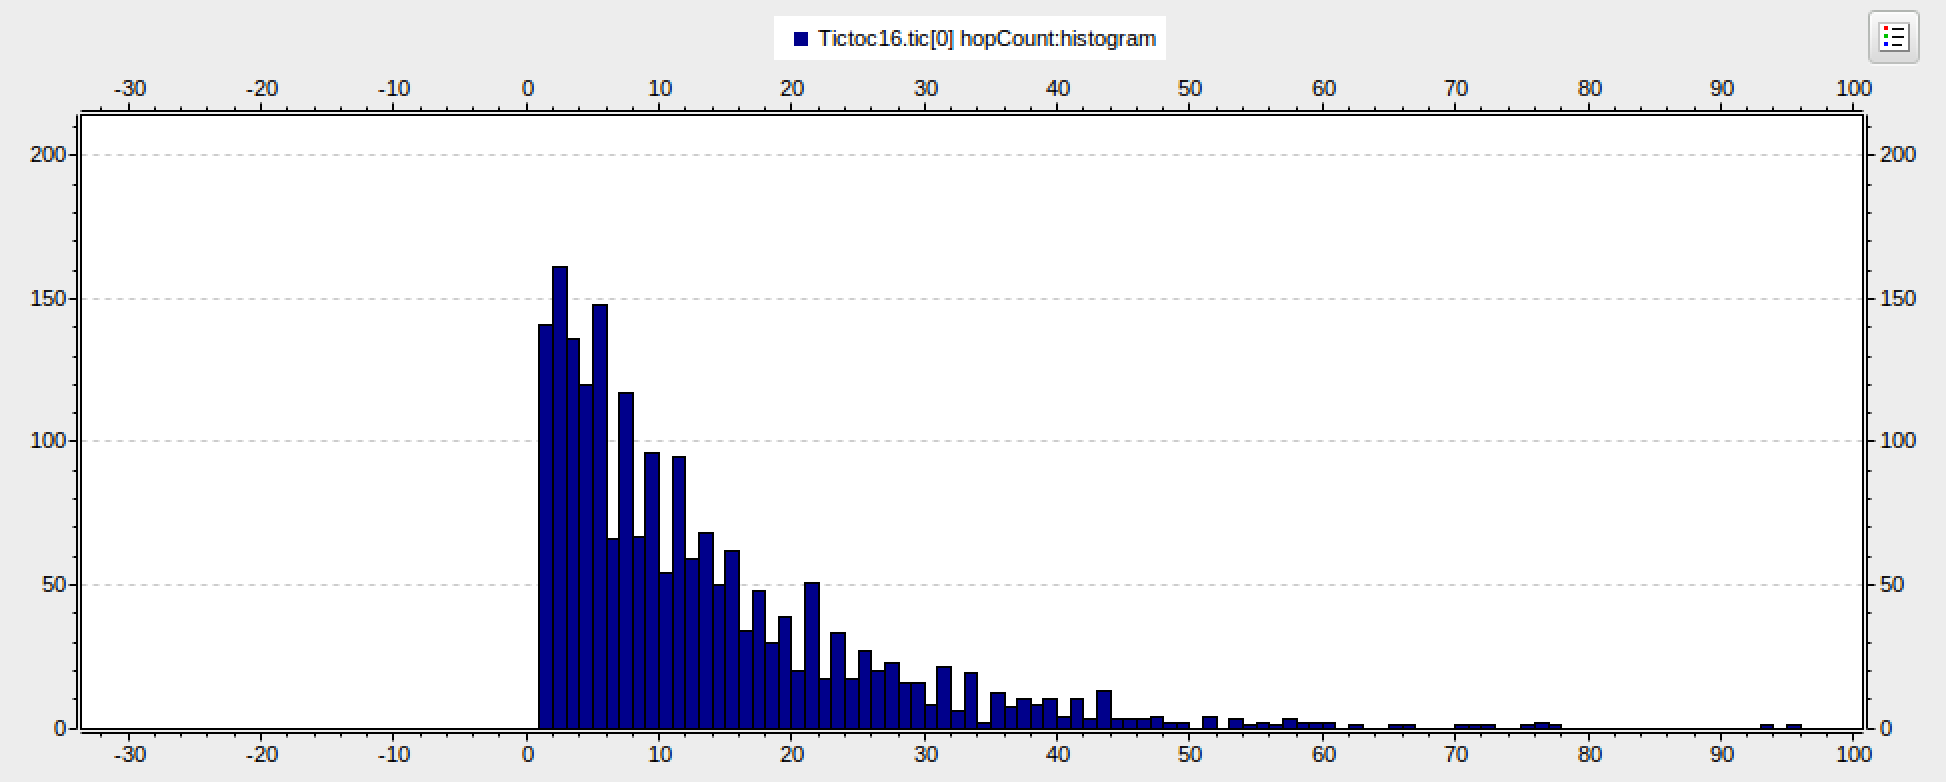
\includegraphics[width=0.9\textwidth]{tictoc16/figura4.png}
			\caption{Histograma tic0 tictoc16}
			\end {figure}
		
		\newpage
		
		\begin{figure}[htb]
			\centering
			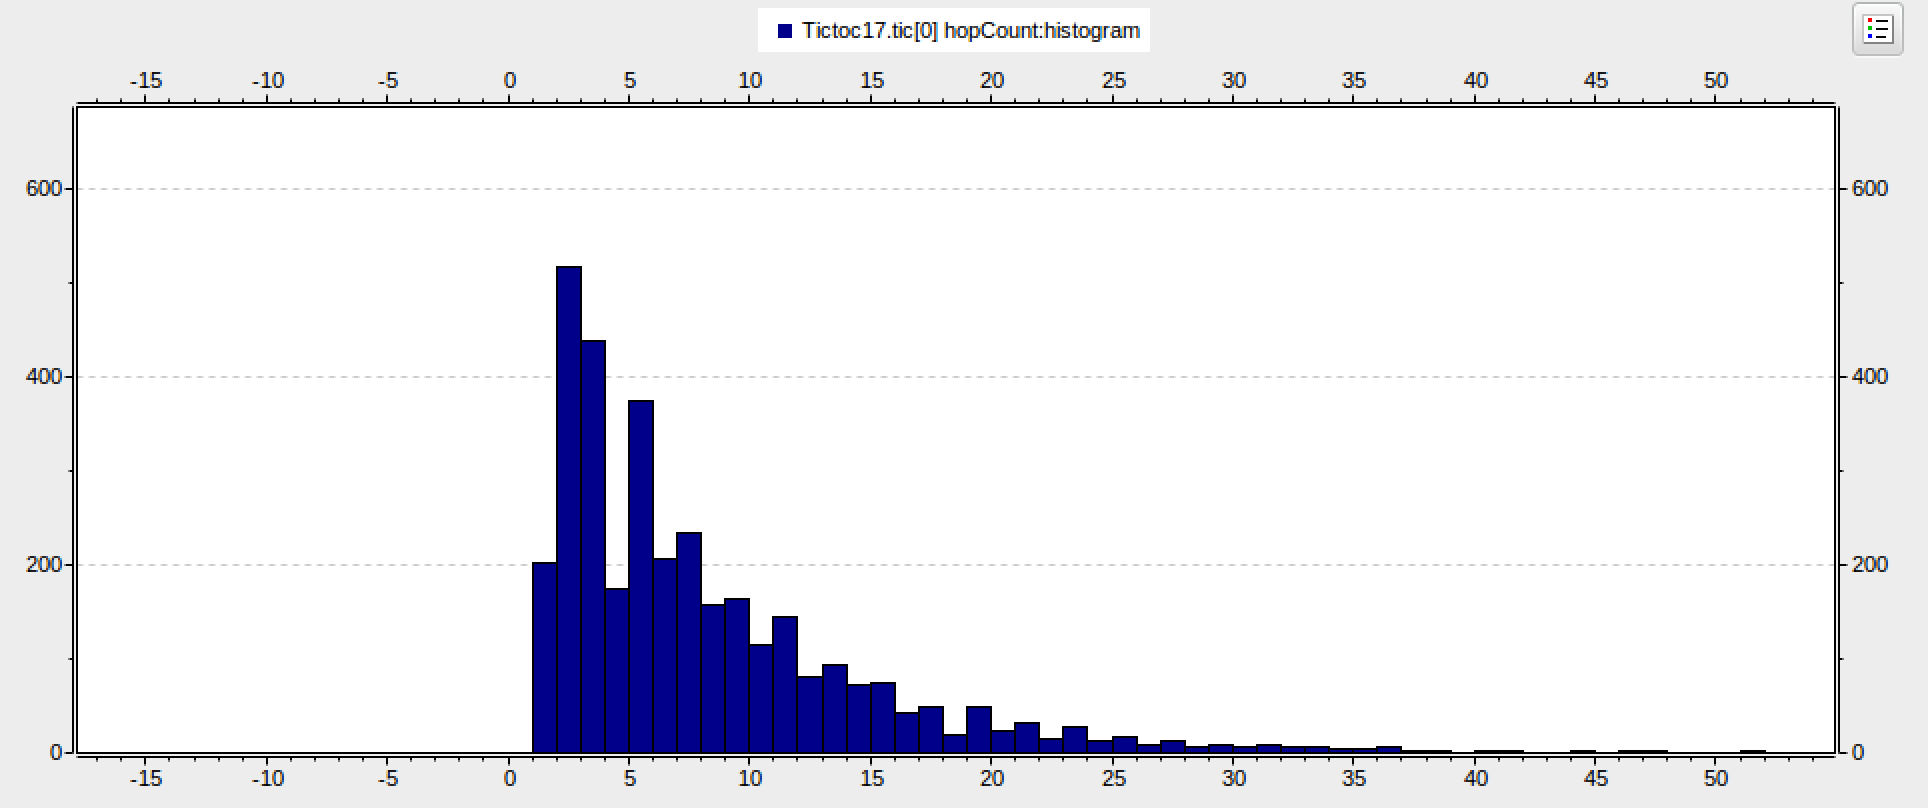
\includegraphics[width=0.9\textwidth]{tictoc17v1/figura4.png}
			\caption{Histograma tic0 tictoc17 version 1}
			\end {figure}		
		
		\begin{figure}[htb]
			\centering
			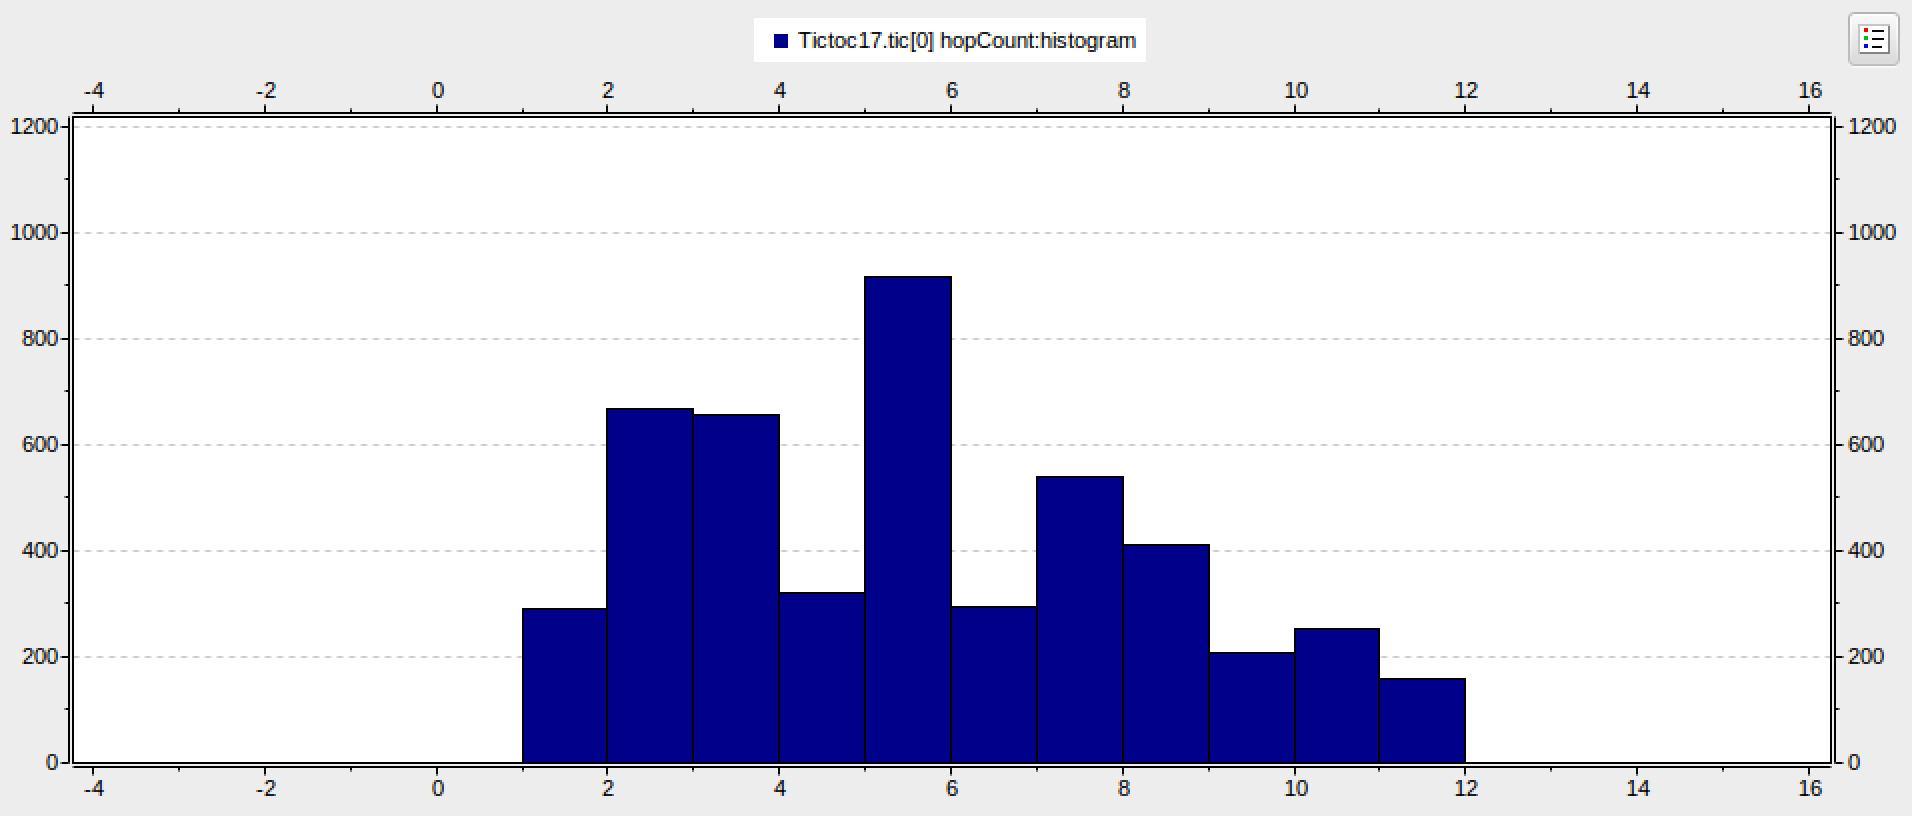
\includegraphics[width=0.9\textwidth]{tictoc17v2/figura4.png}
			\caption{Histograma tic0 tictoc17 version 2}
			\end {figure}
			
			
		Como se ve, con la implementación mejorada un paquete  que tenga como destino un nodo externo solo puede saltar entre 1 y 11 veces. Se aprecia la diferencia ya que se eliminan los bucles respecto a las implementaciones anteriores. 
		También se  puede ver que el máximo número de veces, los saltos que hacen falta para llegar a un nodo externo son 5, que es el pico del histograma.
		
		\newpage
		
		\textbf{Quinta gráfica: histograma con las repeticiones del número de saltos en tic1, nodo intermedio}\\
		
		\begin{figure}[htb]
			\centering
			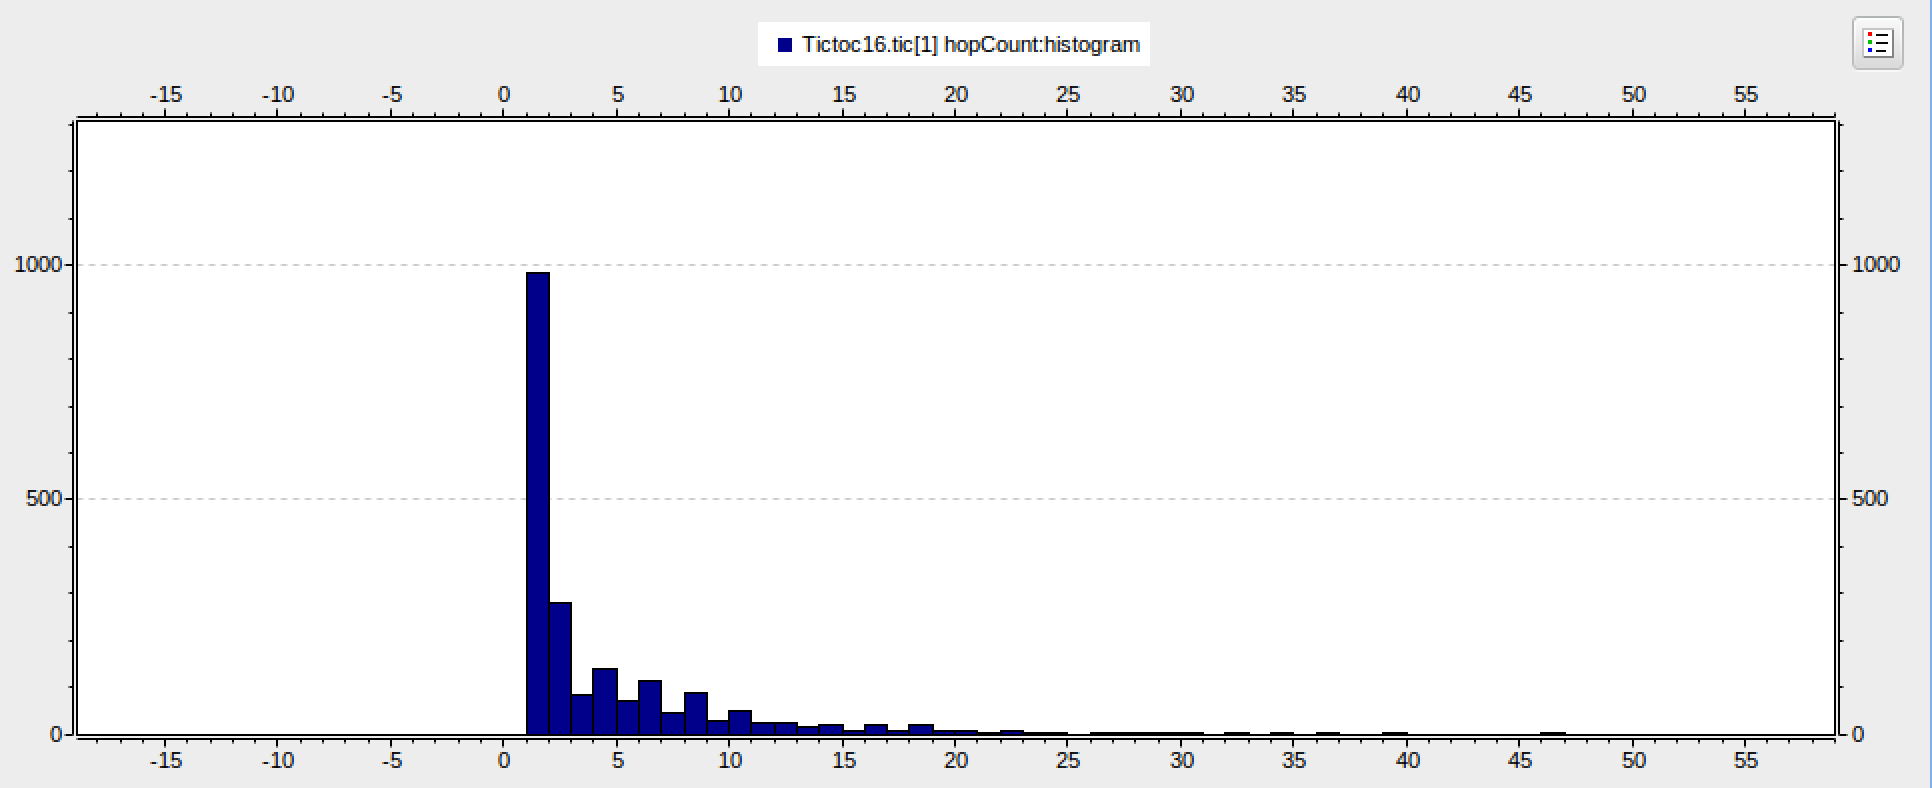
\includegraphics[width=0.9\textwidth]{tictoc16/figura5.png}
			\caption{Histograma tic1 tictoc16}
			\end {figure}
			
		\begin{figure}[htb]
			\centering
			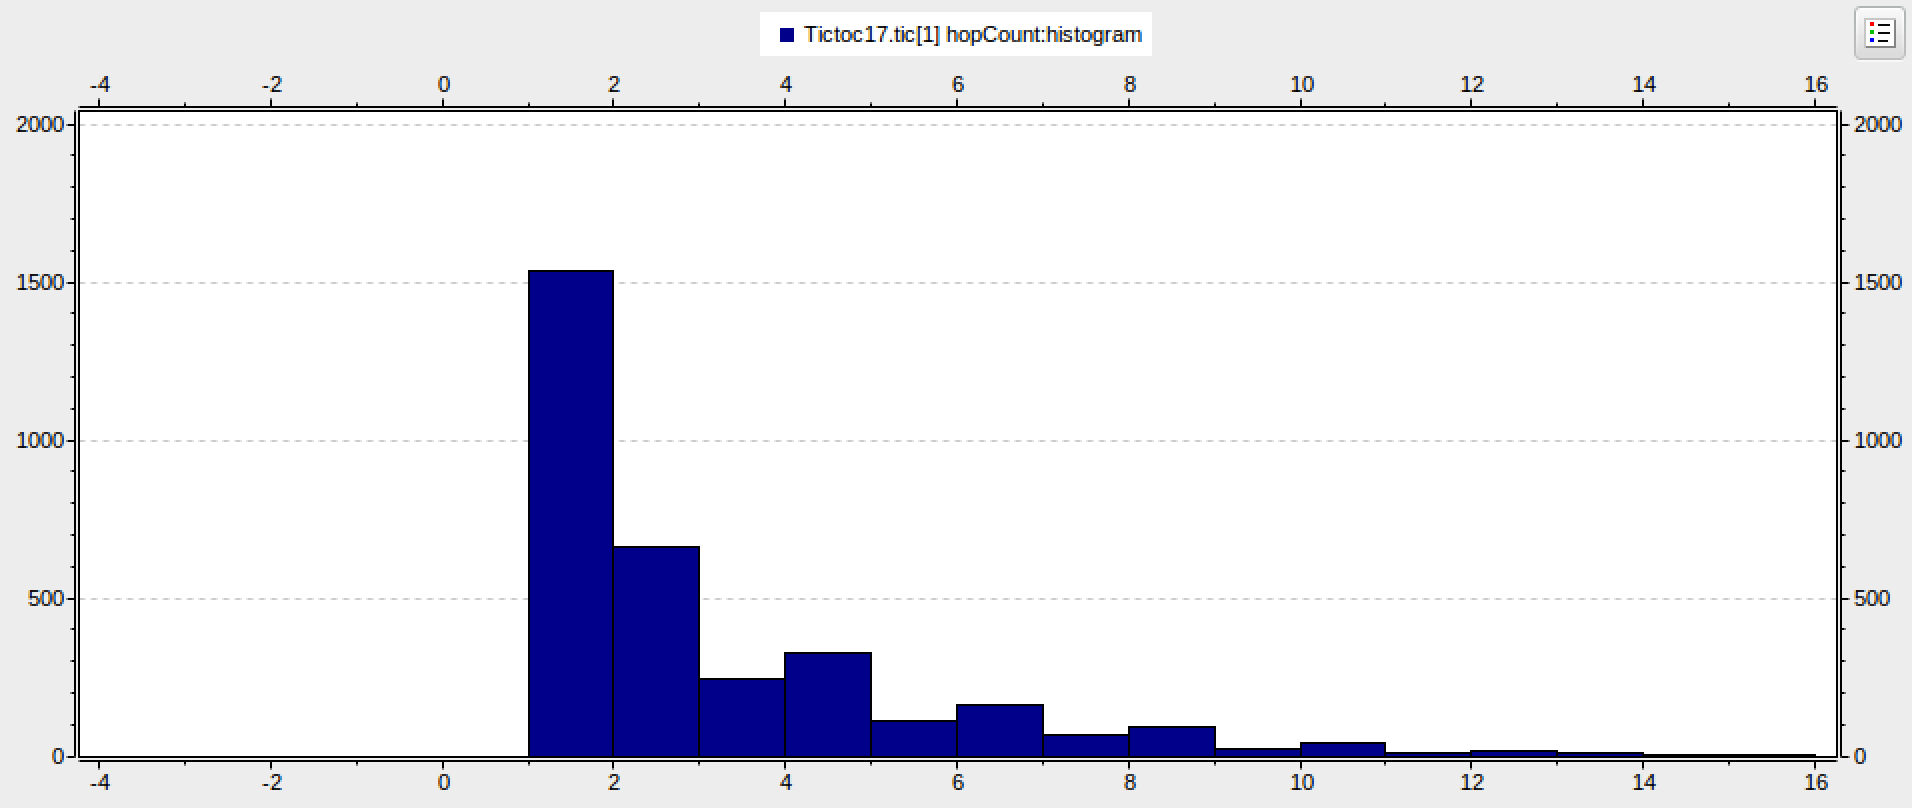
\includegraphics[width=0.9\textwidth]{tictoc17v1/figura5.png}
			\caption{Histograma tic1 tictoc17 version 1}
			\end {figure}
			
		\newpage
			

		
		Con la implementación mejorada un paquete solo puede  saltar entre 1 y 6 veces antes de llegar a un nodo intermedio como es tic1. La mayoría de veces, el paquete solo tardará un salto, que es el pico del histograma. Este comportamiento de solo un salto es similar en las tres gráficas, pero nuestra ultima mejora permite que no haya variaciones tan grandes como por ejemplo 46 saltos antes de llegar, como se ve en la primera gráfica.


	\newpage
	
	\section{Práctica 2}
	
	\subsection{Análisis del funcionamiento de \textit{nclients} }
	
	En el ejemplo nclients se presenta un escenario básico en el que un cliente se conecta a un servidor telnet a través de tres routers intermedios.
	
	Para ello hay definidas dos topologías de red similares, una utlizando Ethernet (NClientsEth.ned), en la que se define un canal ethernetline (delay 0.1 microsegundos, datarate 10 Mbps). La segunda configuración utiliza PPP (NClientsPPP.ned), definiendo un canal fiberline (delay 0.1 microsegundos, datarate 512 Mbps). En el fichero omnetpp.ini hay definidas tres configuraciones. Una de ellas, la configuración ETH, utiliza la definición de red NClientsEth.ned. Las otras dos, PPP y PPP\_SCTP utilizan la definición de red NClientsPPP.ned. La configuración ETH utilizará el protocolo TCP. Por su parte, las configuracion PPP utiliza el protocolo TCP, y la PPP\_SCTP utiliza el protocolo SCTP.
	
	Para analizar el comportamiento del ejemplo, primero se estudiará el comportamiento de la configuración ETH. Cuando se ejecuta el escenario que se muestra es el siguiente: \\
	
			\begin{figure}[htb]
				\centering
				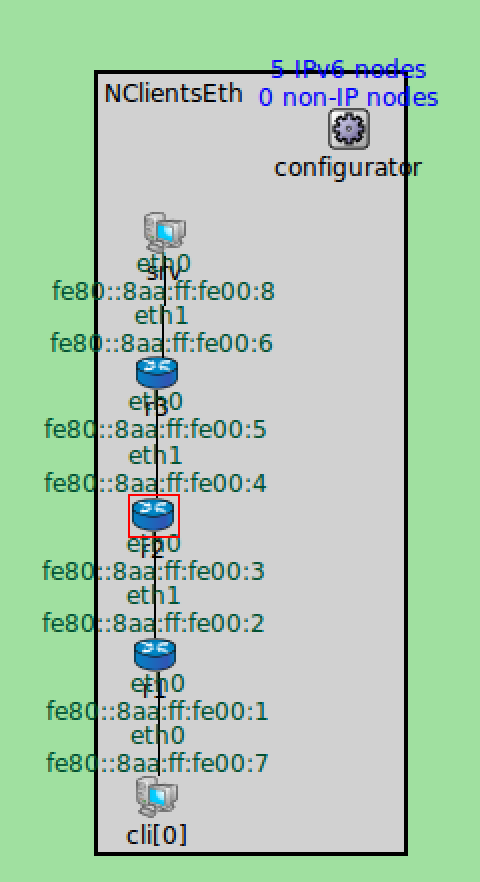
\includegraphics{P2/figura1.png}
				\caption{Esquema de la red del ejemplo ETH}
				\end {figure}		
				
				
				
		
	
\end{document}